\chapter{Introducción}
\label{chap:intro}

\drop{E}{l} guiado de personas es una actividad que se lleva desarrollando desde siempre con la
ayuda de las estrellas, mapas y brújulas. Afortunadamente para nosotros, desde que se desarrolló en
los años sesenta \textit{Transit} considerado el primer \acf{SGNS} o \acf{GNSS}, resulta bastante
más sencillo conocer nuestra ubicación en el globo de forma precisa y seguir un determinado camino.

A pesar de que \textit{Transit} se desarrollase en los años sesenta, no fue hasta 1983 cuando Honda
se planteó utilizar la tecnología de los \acs{SGNS} para guiar a civiles y desarrolló su sistema de
navegación, culminándolo en 1990 para el Honda Legend Acura Legend. Desde entonces se democratizó el
uso de los \acs{SGNS} hasta el punto de encontrar en el mercado un elevado número de \acf{PDA}
equipados con sistemas de navegación a finales de la primera década del 2000.

Con la reciente popularización de los smartphones se ha extendido aún más el uso de la navegación
vía satélite y es común encontrar personas utilizándola por medio de aplicaciones como
\textit{Google Maps}, \textit{iOS Maps} o \textit{Nokia HERE}. Estas aplicaciones
resultan muy útiles ya que nos permiten llegar a cualquier sitio sin necesidad de conocer el camino
previamente pero implican un requisito importante: es necesario ver la pantalla u oír las
instrucciones para llevarlas a cabo. Eso no es demasiado inconveniente en un coche, pero para los
peatones, ciclistas y motoristas el hecho de mirar a la pantalla o intentar oír el smartphone supone
una distracción que potencialmente puede provocar un accidente~\cite{Valcarcel12} y, por tanto, para
hacer uso de la navegación vía satélite necesitan otro tipo de interacción con el dispositivo.

Las distracciones del conductor son una de las principales causas de accidentabilidad a nivel
mundial. La \acf{NHTSA} señaló en 2003 que la distracción de los conductores es la causa de 1,5
millones de accidentes producidos anualmente en todo el planeta \cite{RACC03}. Y, según un estudio
de la aseguradora Allianz de 2014 \cite{Allianz14}, el 26\% de los accidentes producidos por
distracciones se deben a mirar la pantalla del navegador.

Las autoridades de todo el mundo conocen la relación entre distracciones y accidentes e intentan
evitar que se produzcan por medio de su legislación. A día de hoy, en España, el uso de dispositivos
como navegadores, cascos y auriculares por parte del conductor está considerado como una infracción
grave y acarrea una multa de 200 euros y una pérdida de 3 puntos en el carné de conducir
\cite{Serrano14} .

Para hacer frente al problema de las distracciones a la hora de utilizar los sistemas de navegación,
en este trabajo se desarrollará un sistema de guiado en el que el usuario obtendrá realimentación
sin necesidad de ver la pantalla, es decir, por medio de la interacción implícita. Para ello, el
sistema avisará al usuario en el momento que tenga que realizar cualquiera de las posibles acciones:
continuar recto, girar, dar media vuelta, etc.

La  interacción implícita que  se pretende  conseguir con  este trabajo  se llevará  a cabo  por dos
medios:
\begin{itemize}
  \item El \textbf{sonido}. Como todos los navegadores actuales nos proporcionará las instrucciones
    de manera auditiva pero como el trabajo va dirigido a peatones, ciclistas y motoristas y resulta
    complicado escuchar nuestro dispositivo en un ambiente abierto, necesitaremos otra interacción
    adicional.
  \item La \textbf{vibración}. Necesaria para las situaciones en las que resulte complicado oír el
    dispositivo y porque está prohibido el uso de cascos o auriculares.
\end{itemize}

El proyecto pretende utilizar un teléfono (smartphone) y su vibrador junto con un periférico como un
reloj (smartwatch) o pulsera inteligente (smartband). De este modo, cuando haya que girar a la
izquierda vibrará uno, cuando haya que girar a la derecha vibrará el otro y cuando haya que dar
media vuelta vibrarán ambos. De esta manera, si nos colocamos el smartwatch o smartband en la mano
izquierda y el teléfono en el bolsillo derecho, cuando tengamos que realizar un giro a la izquierda
solamente vibrará el complemento dejando evidente la acción a realizar (ver
Figura~\ref{fig:giroIzquierda}).

\begin{figure}[!h]
  \begin{center}
    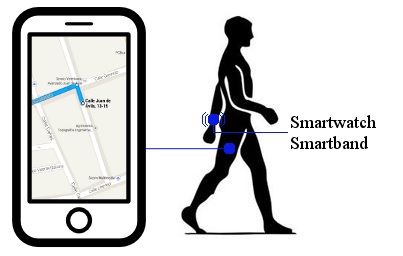
\includegraphics[width=0.65\textwidth]{/esquema-giro-izquierda.png}
    \caption{Ejemplo del sistema girando a la izquierda}
    \label{fig:giroIzquierda}
  \end{center}
\end{figure}


\section{Estructura del documento}

A continuación se detalla la estructura de este documento para facilitar la lectura del mismo y
se describe brevemente el contenido de cada uno de los capítulos que lo componen.

\begin{definitionlist}
  \item[Capítulo \ref{chap:objetivos}: \nameref{chap:objetivos}] 

  El principal objetivo de este proyecto es el diseño e implementación de un sistema de navegación
  por satélite que se comunique con el usuario por medio de la vibración de alguno de sus
  componentes.

  En este capítulo se detallan los objetivos específicos que se pretenden alcanzar a lo largo del
  desarrollo del proyecto y las limitaciones asociadas.

  \item[Capítulo \ref{chap:antecedentes}: \nameref{chap:antecedentes}]

  En este capítulo se hace una introducción al concepto de interacción implícita. También se hace un
  repaso de los diferentes sistemas de navegación vía satélite y las aplicaciones para
  smartphone. Se pondrá especial interés en la forma que tienen para comunicarse con sus usuarios.

  Además, se realizarán estudios que nos permita realizar buenas elecciones a lo largo del \acs{TFG}
  sobre las plataformas de smartphones, los complementos vibratorios y los proveedores de mapas y
  rutas existentes en la actualidad.

  \item[Capítulo \ref{chap:metodo}: \nameref{chap:metodo}]

  En este capítulo se describe la metodología seguida, además de especificar las herramientas,
  tanto hardware como software, utilizadas para la elaboración de este proyecto.

  \item[Capítulo \ref{chap:desarrollo}: \nameref{chap:desarrollo}]

  En este capitulo se encuentra detallado el trabajo realizado especificando cada una de las
  iteraciones necesarias para el desarrollo del proyecto.

  \item[Capítulo \ref{chap:resultados}: \nameref{chap:resultados}]

  En este capítulo se describen los resultados obtenidos tras el desarrollo del sistema y se hablará
  sobre los recursos y costes del sistema, es decir, medidas de rendimiento y estadísticas recogidas
  del mismo.

  \item[Capítulo \ref{chap:conclusiones}: \nameref{chap:conclusiones}]

  En este capítulo se detallarán las conclusiones obtenidas del desarrollo del proyecto, se
  incluirán posibles usos alternativos del sistema y se propondrán posibles líneas de trabajo
  futuras a desarrollar.

\end{definitionlist}

% Local Variables:
%  TeX-master: "main.tex"
%  coding: utf-8
%  mode: latex
%  mode: flyspell
%  ispell-local-dictionary: "castellano8"
% End:
